\begin{figure}[h]
   \centering
   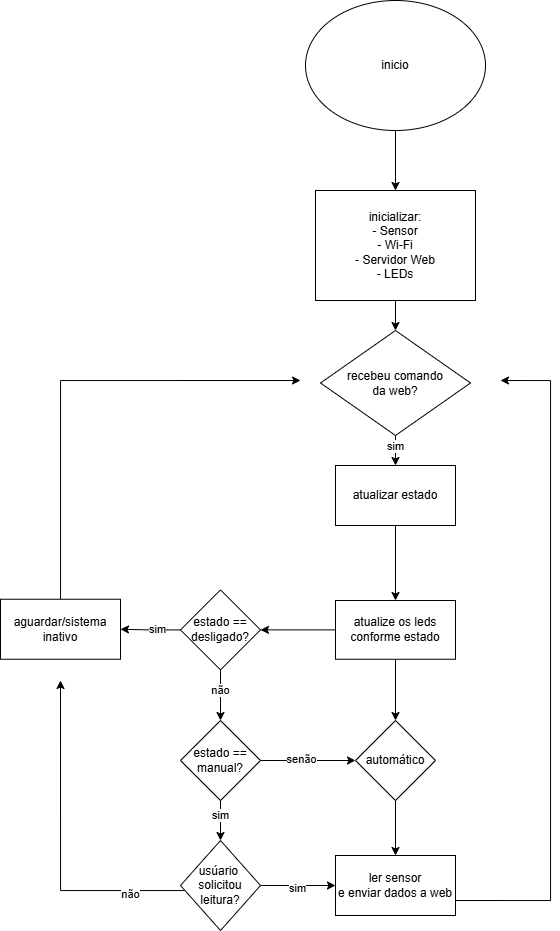
\includegraphics[width=0.6\textwidth]{imagens/fluxograma2.png} 
    \caption{Fluxograma do software do leitor de temperatura}
    \label{fig:fluxograma_software}
\end{figure}

\subsection{Descrição do Fluxograma do Software}

O fluxograma desenvolvido representa a lógica de funcionamento do software embarcado responsável pelo monitoramento de temperatura e umidade, bem como a interação com a interface web e o controle dos LEDs indicadores de estado.

Inicialmente, o sistema realiza a etapa de inicialização, na qual são configurados todos os periféricos necessários para o funcionamento do projeto. Nessa etapa, são inicializados o sensor de temperatura e umidade, o módulo de comunicação Wi-Fi, o servidor web responsável pela interface com o usuário e os pinos de controle dos LEDs. Após a inicialização, o sistema define seu estado inicial como \textbf{Desligado}.

Em seguida, o sistema entra em um \textbf{loop principal de execução contínua}, característica fundamental de sistemas embarcados. Nesse loop, todas as operações do sistema são realizadas de forma cíclica e ininterrupta.

A cada iteração do loop, o sistema verifica se há novos comandos provenientes da interface web. Caso um comando seja recebido, o estado do sistema é atualizado de acordo com a solicitação do usuário, permitindo a alternância entre os modos de operação: Desligado, Manual e Automático. Caso não haja comando, o sistema mantém o estado atual.

Após a possível atualização do estado, os LEDs indicadores são atualizados para refletir o modo de operação vigente, fornecendo uma indicação visual clara do estado do sistema.

\begin{itemize}
\item \textbf{Modo Desligado:}
Neste estado, o sistema permanece inativo, não realizando leituras do sensor nem enviando dados para a interface web. O sistema apenas mantém o loop ativo, aguardando novos comandos do usuário.

\item \textbf{Modo Manual:}  
No modo manual, o sistema aguarda uma solicitação explícita do usuário para realizar a leitura dos dados. Caso o usuário solicite a leitura por meio da interface web, o sistema realiza a coleta dos dados do sensor e os envia para exibição. Caso contrário, permanece em espera, sem executar novas leituras.

\item \textbf{Modo Automático:}  
Neste modo, o sistema realiza leituras periódicas do sensor de forma contínua e automática. Após cada leitura, os dados de temperatura e umidade são enviados à interface web. Um intervalo de tempo é aplicado entre as leituras para evitar sobrecarga do sistema e garantir estabilidade na aquisição dos dados.

\end{itemize}

Independentemente do modo de operação, ao final de cada ciclo de execução, o sistema retorna ao início do loop principal, reiniciando o processo de verificação de comandos e execução das ações correspondentes. Esse comportamento garante a operação contínua e responsiva do sistema.

Dessa forma, o fluxograma representa de maneira clara e estruturada o funcionamento do software, evidenciando a separação entre inicialização, controle de estados, interação com o usuário e execução das funcionalidades principais do sistema.